%------------------------------ ASSUMPTIONS AND APPROXIMATIONS ------------------------------%
Table \ref{tab:assumptions} contains assumptions and approximations about the working conditions and applied loads.
\begin{table}[H]
    \centering
    \caption{Assumptions Made During Robot Modelling}
    \label{tab:assumptions}
    \begin{tabular}{l l}
        \\ \hline
        \textbf{Assumption Type} & \textbf{Assumption} 
        \\ \hline
        Maximum slope angle & $20^{\circ}$
        \\
        Maximum wind speed & 73 km/h (Ottawa, September 2018 Tornadoes)
        \\
        Linkage composition & Homogeneous rigid bodies
        \\
        Terrain & Sand, pebble, shallow water (under chassis), mud, small plants
        \\
        Environment & Salt, dust, high heat, humidity
        \\ \hline
    \end{tabular}
\end{table}

The maximum slope angle was found as the largest angle for which the robot is still stable.


%------------------------------ External Forces Scenarios ------------------------------%
\subsection{External Forces} \label{sec:modelling_slope}
The defining forces are external forces applied at various locations on the limbs of the robots, mainly normal forces and friction forces which are applied at the extremities of the limbs. Different environmental scenarios encountered by the robot have an impact on the magnitude and direction of these external forces. 

The robot must resist two types of soil slope, one around the $x$ axis and the other around the $y$ axis as shown in Figure \ref{fig:mod_Slope_XY}.

\begin{figure}
    \centering
    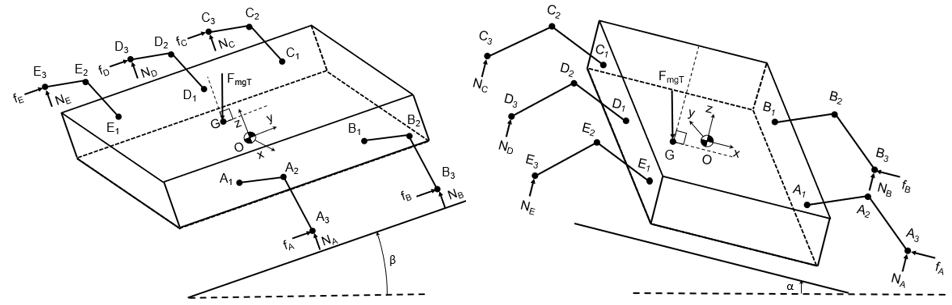
\includegraphics[width=\textwidth]{3_SystemModelling/img/Slope_XY.PNG}
    \caption{Slope Worst Case Scenarios: Around X (Left) and Around Y (Right)}
    \label{fig:mod_Slope_XY}
\end{figure}

The robot will have three legs touching the ground at all times in two different possible leg configuration: ACD and BDE, these were determined by the stability analysis found in section \ref{sec:analysis}. The worst case scenario were assumed for both slope scenarios and shown in Figure \ref{fig:mod_Slope_XY}. For a slope around the $x$ axis, the worst case combination is ACD. For a slope around $y$ axis, both leg combinations are worst case scenarios as long as only one leg is situated at the lower end of the slope. By analysing both scenarios, the following assumptions were made for easier calculations.

Assumptions for slope around $x$ axis.
\begin{enumerate}
  \item Friction force only acts on the two lowest legs
  \item No slipping
\end{enumerate}

Assumptions for slope around $y$ axis.
\begin{enumerate}
  \item Friction force only acts on the lowest leg 
\item No slipping
\end{enumerate}

A visual analysis of both scenarios demonstrates that the friction force will have negligible to beneficial impact on the torque of the motors. For a slope around $x$ axis, the friction will affect the shaft and bearing calculations. For the slope around the $y$ axis, the friction force will counter the torque created by the normal force thus being beneficial to the motor. As discussed later in Section \ref{subsec:Tspring} the robot is now equipped with springs to reduce the torque when static. Due to the spring, the friction force will now have a negative impact on the motor. However, this impact will mostly impact the energy required for the robot to standstill. 

\subsubsection{Normal Forces}
The 2 combinations of feet touching the ground are: 1. A, C, D and 2. B, D, E. To simplify calculations and algebra, a matrix system approach was used. 

For combination 1., the sum of forces and moments are given by
\begin{gather}
    \sum F_z = 0 = N_A + N_C + N_D - F_{mgT}
    \\
    \sum M_{A_x} = 0 = N_C r_{ca_y} + N_D r_{da_y} - F_{mgT} r_{ga_y}
    \\
    \sum M_{C_y} = 0 = -N_A r_{ac_x} -N_D r_{dc_x} + F_{mgT} r_{gc_x}
\end{gather}

For combination 2., the sum of forces and moments are given by
\begin{gather}
    \sum F_z = 0 = N_B + N_D + N_E - F_{mgT}
    \\
    \sum M_{B_x} = 0 = -N_D r_{db_y} - N_E r_{eb_y} + F_{mgT} r_{gb_y}
    \\
    \sum M_{E_y} = 0 = -N_B r_{be_x} -N_D r_{de_x} + F_{mgT} r_{ge_x}
\end{gather}

where the $r$ values represent the distance between the foot and the reference point, perpendicular to the rotation axis. To calculate the distance between two points, cartesian coordinates were used, these can be found in Appendix \ref{app:coordinate}.

The following is an example with combination 1. A matrix solver is used to find reaction values.

\begin{equation}
\begin{split}
    \left[ \begin{array}{ccc} 
    N_A 
    \\ 
   N_C
    \\ 
    N_D
    \end{array} \right]= \left[ \begin{array}{ccc} 
    1 & 1 & 1 
    \\ 
    0 & r_{ca_y} & r_{da_y} 
    \\ 
    r_{ac_x} & r_{dc_x} & 0
    \end{array} \right]^{-1}
    \left[ \begin{array}{ccc} 
    F_{mgT}
    \\ 
    F_{mgT} r_{ga_y} 
    \\ 
    F_{mgT} r_{gc_x}
    \end{array} \right] 
    \\ 
   = \left[ \begin{array}{ccc} 
    1 & 1 & 1 
    \\ 
    0 & 600 mm & 200mm 
    \\ 
    1137mm & 0 & 0
    \end{array} \right]^{-1}
    \left[ \begin{array}{ccc} 
    302N
    \\ 
    60443Nmm
    \\ 
    180118Nmm
    \end{array} \right] 
    = 
    \left[ \begin{array}{ccc} 
    158N
    \\ 
    79N
    \\ 
    64N
    \end{array} \right] 
\end{split}
\end{equation}

The equations are modified to include a slope factor as shown in Equation \ref{eq:normal_forces_slopes}, the normal forces are found when the robot is subject to a slope. Figure \ref{fig:mod_force_slope} shows the normal force for every leg of a combination when subjected to a slope around the y-axis.

\begin{equation}
\begin{split}
    \left[ \begin{array}{ccc} 
    N_A 
    \\ 
   N_C
    \\ 
    N_D
    \end{array} \right]= \left[ \begin{array}{ccc} 
    1 & 1 & 1 
    \\ 
    0 & r_{ca_y} & r_{da_y} 
    \\ 
    r_{ac_x} & r_{dc_x} & 0
    \end{array} \right]^{-1}
    \left[ \begin{array}{ccc} 
    F_{mgT} \cos{Slope}
    \\ 
    F_{mgT} r_{ga_y} \cos{Slope}
    \\ 
    F_{mgT} (r_{gc_x}\cos{Slope} - r_{gc_z}\sin{Slope} )
    \end{array} \right] 
\end{split}\label{eq:normal_forces_slopes}
\end{equation} 


\begin{figure}
    \centering
    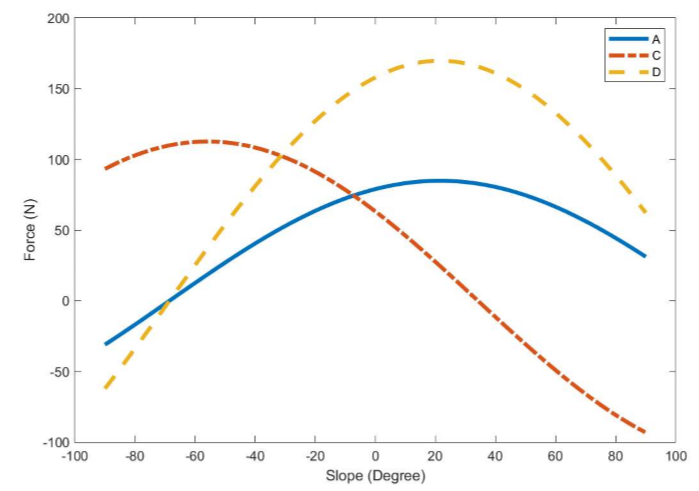
\includegraphics[width=0.5\textwidth]{3_SystemModelling/img/SlopeForces.PNG}
    \caption{Normal Force for all slope angles around y-axis}
    \label{fig:mod_force_slope}
\end{figure}

\subsubsection{Friction Force - Slope around X axis}
For this type of slope, the lowest leg on each side of the robot will be subject to friction, for combination of leg ACD, Leg A and Leg D will be subject to friction. The slope of 20 degrees was determined and explained in Section \ref{sec:stability}.

\begin{gather}
\begin{split}
    \sum M_{A_z} = 0 = -F_D r_{D \rightarrow A} + F_{mgt} \sin{\beta} r_{CG \rightarrow A} 
    \\
    \rightarrow F_D = \frac{F_{mgt} \sin{\beta} r_{CG \rightarrow A}}{r_{D \rightarrow A}} = \frac{(299.99N) \sin{(20 deg)} (1136mm-596mm)}{(1136mm-0mm)} = 48.6 N
\end{split}
    \\
    \begin{split}
        \sum F_y = 0 = F_A + F_D - F_{mgt} \sin{\beta}
        \\
        \rightarrow F_A = F_{mgt}\sin{\beta} - F_D =  (299.99N)\sin{(20 deg)} - (48.6 N) = 54.01 N
    \end{split}
\end{gather}

\subsubsection{Friction Force - Slope around y axis}
Due to the assumptions for a slope around $y$ axis, the friction force $F_A$ (for the case of the leg combination ACD) is the totality of the force transfered as shown in Equation \ref{eq:mod_slope_y_axis}. The slope of 20 degrees was determined and explained in Section \ref{sec:stability}.

\begin{equation}
    F_A = F_{mgT}\sin{\alpha} = (299.99N)\sin{20} = 102.6 N
    \label{eq:mod_slope_y_axis}
\end{equation}


%------------------------------ DYNAMIC EQUATION ------------------------------%
\subsection{Dynamic Equation}

For both the static and dynamic case where the legs are moving, the joint torques are found by developing an inertial matrix, force and gravity matrices, and combining them in the dynamic equation developed in the Robotics course, MCG4134 \cite{al-jarrah_mcg4134:_2019}.
The final form, following derivations presented in the Modelling Report, is given by Equation \ref{eq:dynamic_equation}

\begin{equation} \label{eq:dynamic_equation}
    \begin{split}
        \begin{bmatrix} 
            (m_1 + m_2) L^2 & m_2 \ell L \cos(\theta-\phi) \\
            m_2 \ell L \cos(\theta-\phi) & m_2 \ell
        \end{bmatrix}
        \begin{bmatrix} \Ddot{\theta} \\ \Ddot{\phi} \end{bmatrix}
        -
        g \begin{bmatrix}
            (m_1 + m_2) L \cos\theta + m_2 \ell \cos\theta \\
            m_2 \ell \cos\phi
        \end{bmatrix} \\
        +
        N \begin{bmatrix}
            L\cos\theta + \ell\cos\phi \\
            \ell\cos\phi
            \end{bmatrix} - f \begin{bmatrix}
            L\sin\theta + \ell\sin\phi \\
            \ell\sin\phi
        \end{bmatrix}
        =
        \begin{bmatrix}
        \tau_1 \\ \tau_2
        \end{bmatrix}
    \end{split}
\end{equation}

where $m_1$ and $m_2$ are the masses of the linkages and joints (moved to the most distal point of the linkage), $N$ is the normal force at the foot, $f$ is the friction force at the foot (and encompasses wind, chassis acceleration, and other external forces parallel the ground), and $\tau_1$ and $\tau_2$ are the joint torques at the hip and knee respectively.
This approach is conservative, as the actual inertial matrix would contain mass values closer to the center of the linkages.

As the foot location moves throughout a leg cycle, the torque for both knee and hip motors also fluctuate as shown in Figure \ref{fig:mod_torque_cycle}, where the the torque is plotted over the foot's distance from the hip motor. The torque was calculated using the dynamic equation.
Torsion springs were added later to the robot to reduce the power consumption when in an idle position; the torques before and after adding torsion springs are found in Figures \ref{fig:torque_comparison_hip} and \ref{fig:torque_comparison_knee}.
It can be seen that, during the last third of the cycle, the leg is on the ground and pulling the robot forward; with the torsion springs, the torque is below the backdriving torque of the Harmonic Drives, and so the motors should not consume any power.

\begin{figure}
    \centering
    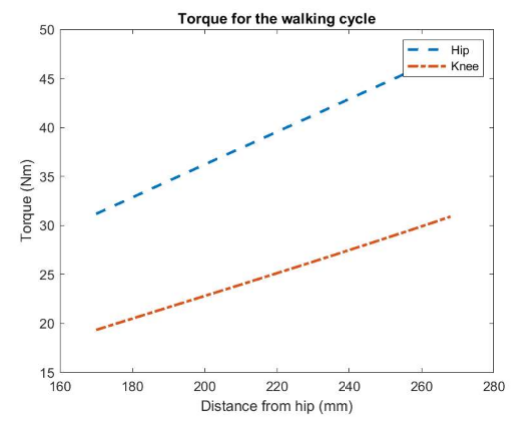
\includegraphics[width=0.5\textwidth]{3_SystemModelling/img/Torque_Cycle.PNG}
    \caption{Torque over the foot's distance from the hip motor.}
    \label{fig:mod_torque_cycle}
\end{figure}

\begin{figure}
    \centering
    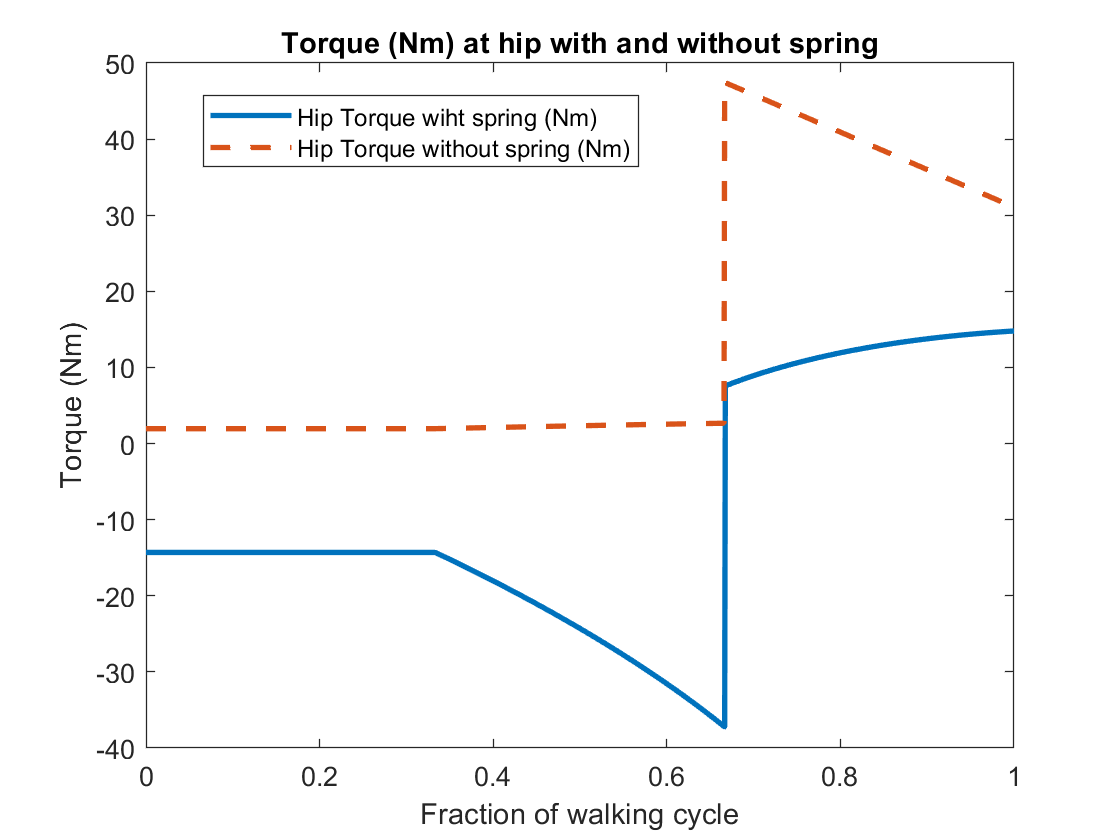
\includegraphics[width=0.5\textwidth]{3_SystemModelling/img/PowerHipComparison.png}
    \caption{Torque at hip joint before and after adding torsion spring}
    \label{fig:torque_comparison_hip}
\end{figure}{}

\begin{figure}
    \centering
    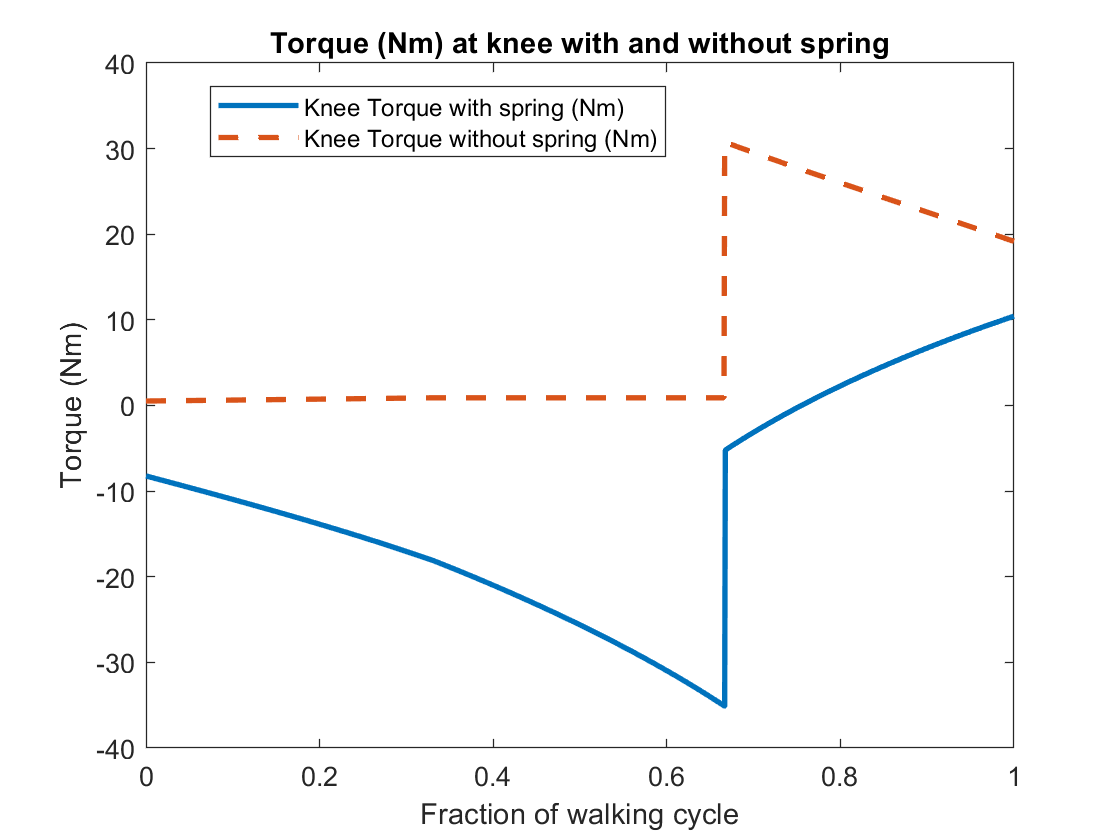
\includegraphics[width=0.5\textwidth]{3_SystemModelling/img/PowerKneeComparison.png}
    \caption{Torque at knee joint before and after adding torsion spring}
    \label{fig:torque_comparison_knee}
\end{figure}{}

%------------------------------ Stability ------------------------------%
\subsection{Stability} \label{sec:stability}
To determine the maximum terrain operating slope, the centre of mass was determined for all three directions, x, y, and z. By connecting the feet for each combination of legs touching the ground simultaneously, stability triangles are created and then used to visually determine an area of stability for both leg combination. The triangle of stability for combination ACD and BDE, the area of stability and the optimal location for the centre of mass is shown in Figure \ref{fig:stability}. For the robot to stay stable during all phases of the walking cycle, the centre of mass must remain in the area of stability. When the robot is subjected to a terrain slope, the different height of the centre of mass (in z direction) will cause the centre of mass to "move" closer to the edges of the area of stability. By using rotational matrices previously presented in the modelling report, the maximum slopes were determined. It was determined that an angle of 20 degrees and -20 degrees around the x and y axis will enable the robot to move properly in one or both slopes. 

\begin{figure}
    \centering
    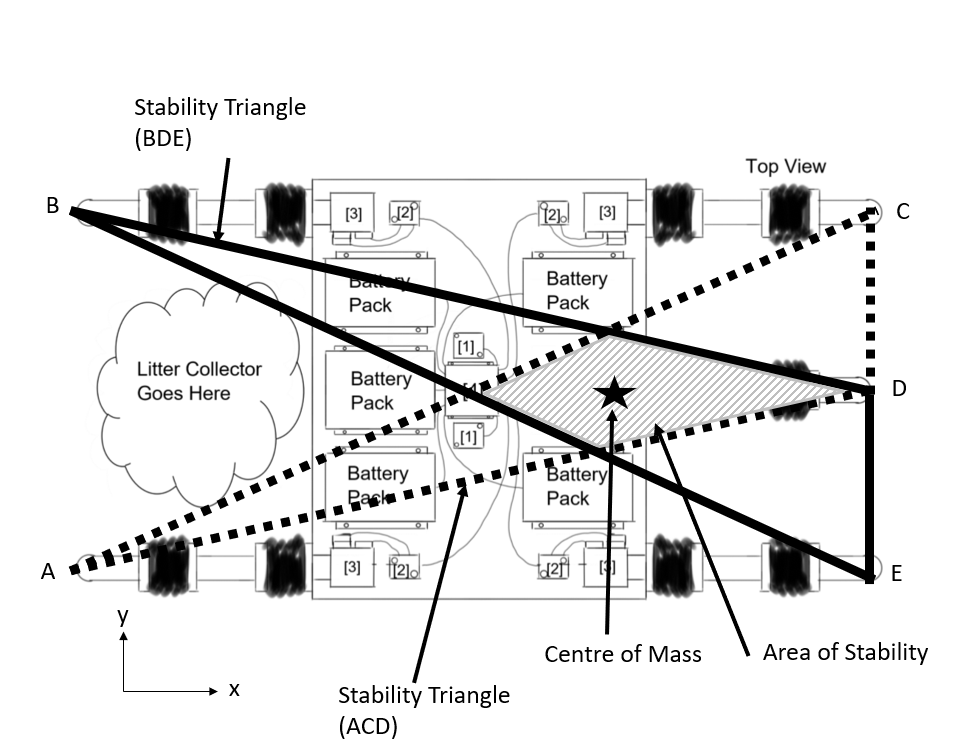
\includegraphics[width=0.7\textwidth]{3_SystemModelling/img/Stability.PNG}
    \caption{Stability Visualization}
    \label{fig:stability}
\end{figure}


%------------------------------ LINKAGE OPTIMIZATION ------------------------------%
\subsection{Linkage Optimization} \label{subsec:linkage_optimization}

In order to determine the relative lengths of the leg linkages, as well as the bend angle in the lower member/tibia, a simple simulation was performed.
First, the range of $\theta$ is between $0^{\circ}$ and $45^{\circ}$ with the body reference frame, shown in Figure \ref{fig:linkage_optimization_diagram}.
Then, the range of $\psi$ is between $-22.5^{\circ}$ and $22.5^{\circ}$ relative to the thigh linkage (this ensures half of the $45^{\circ}$ range above or below the thigh). These values were chosen while considering the limited range of bellows and optimal stability.
The length of $r_1$ is 100mm, and combined length of $r_2$ and $r_3$ is 350mm.
The relative ratio of $r_1$ to $r_2 + r_3$ was determined through trial and error (and would have required more sophisticated methods to determine than the one presented below).

\begin{figure}
    \centering
    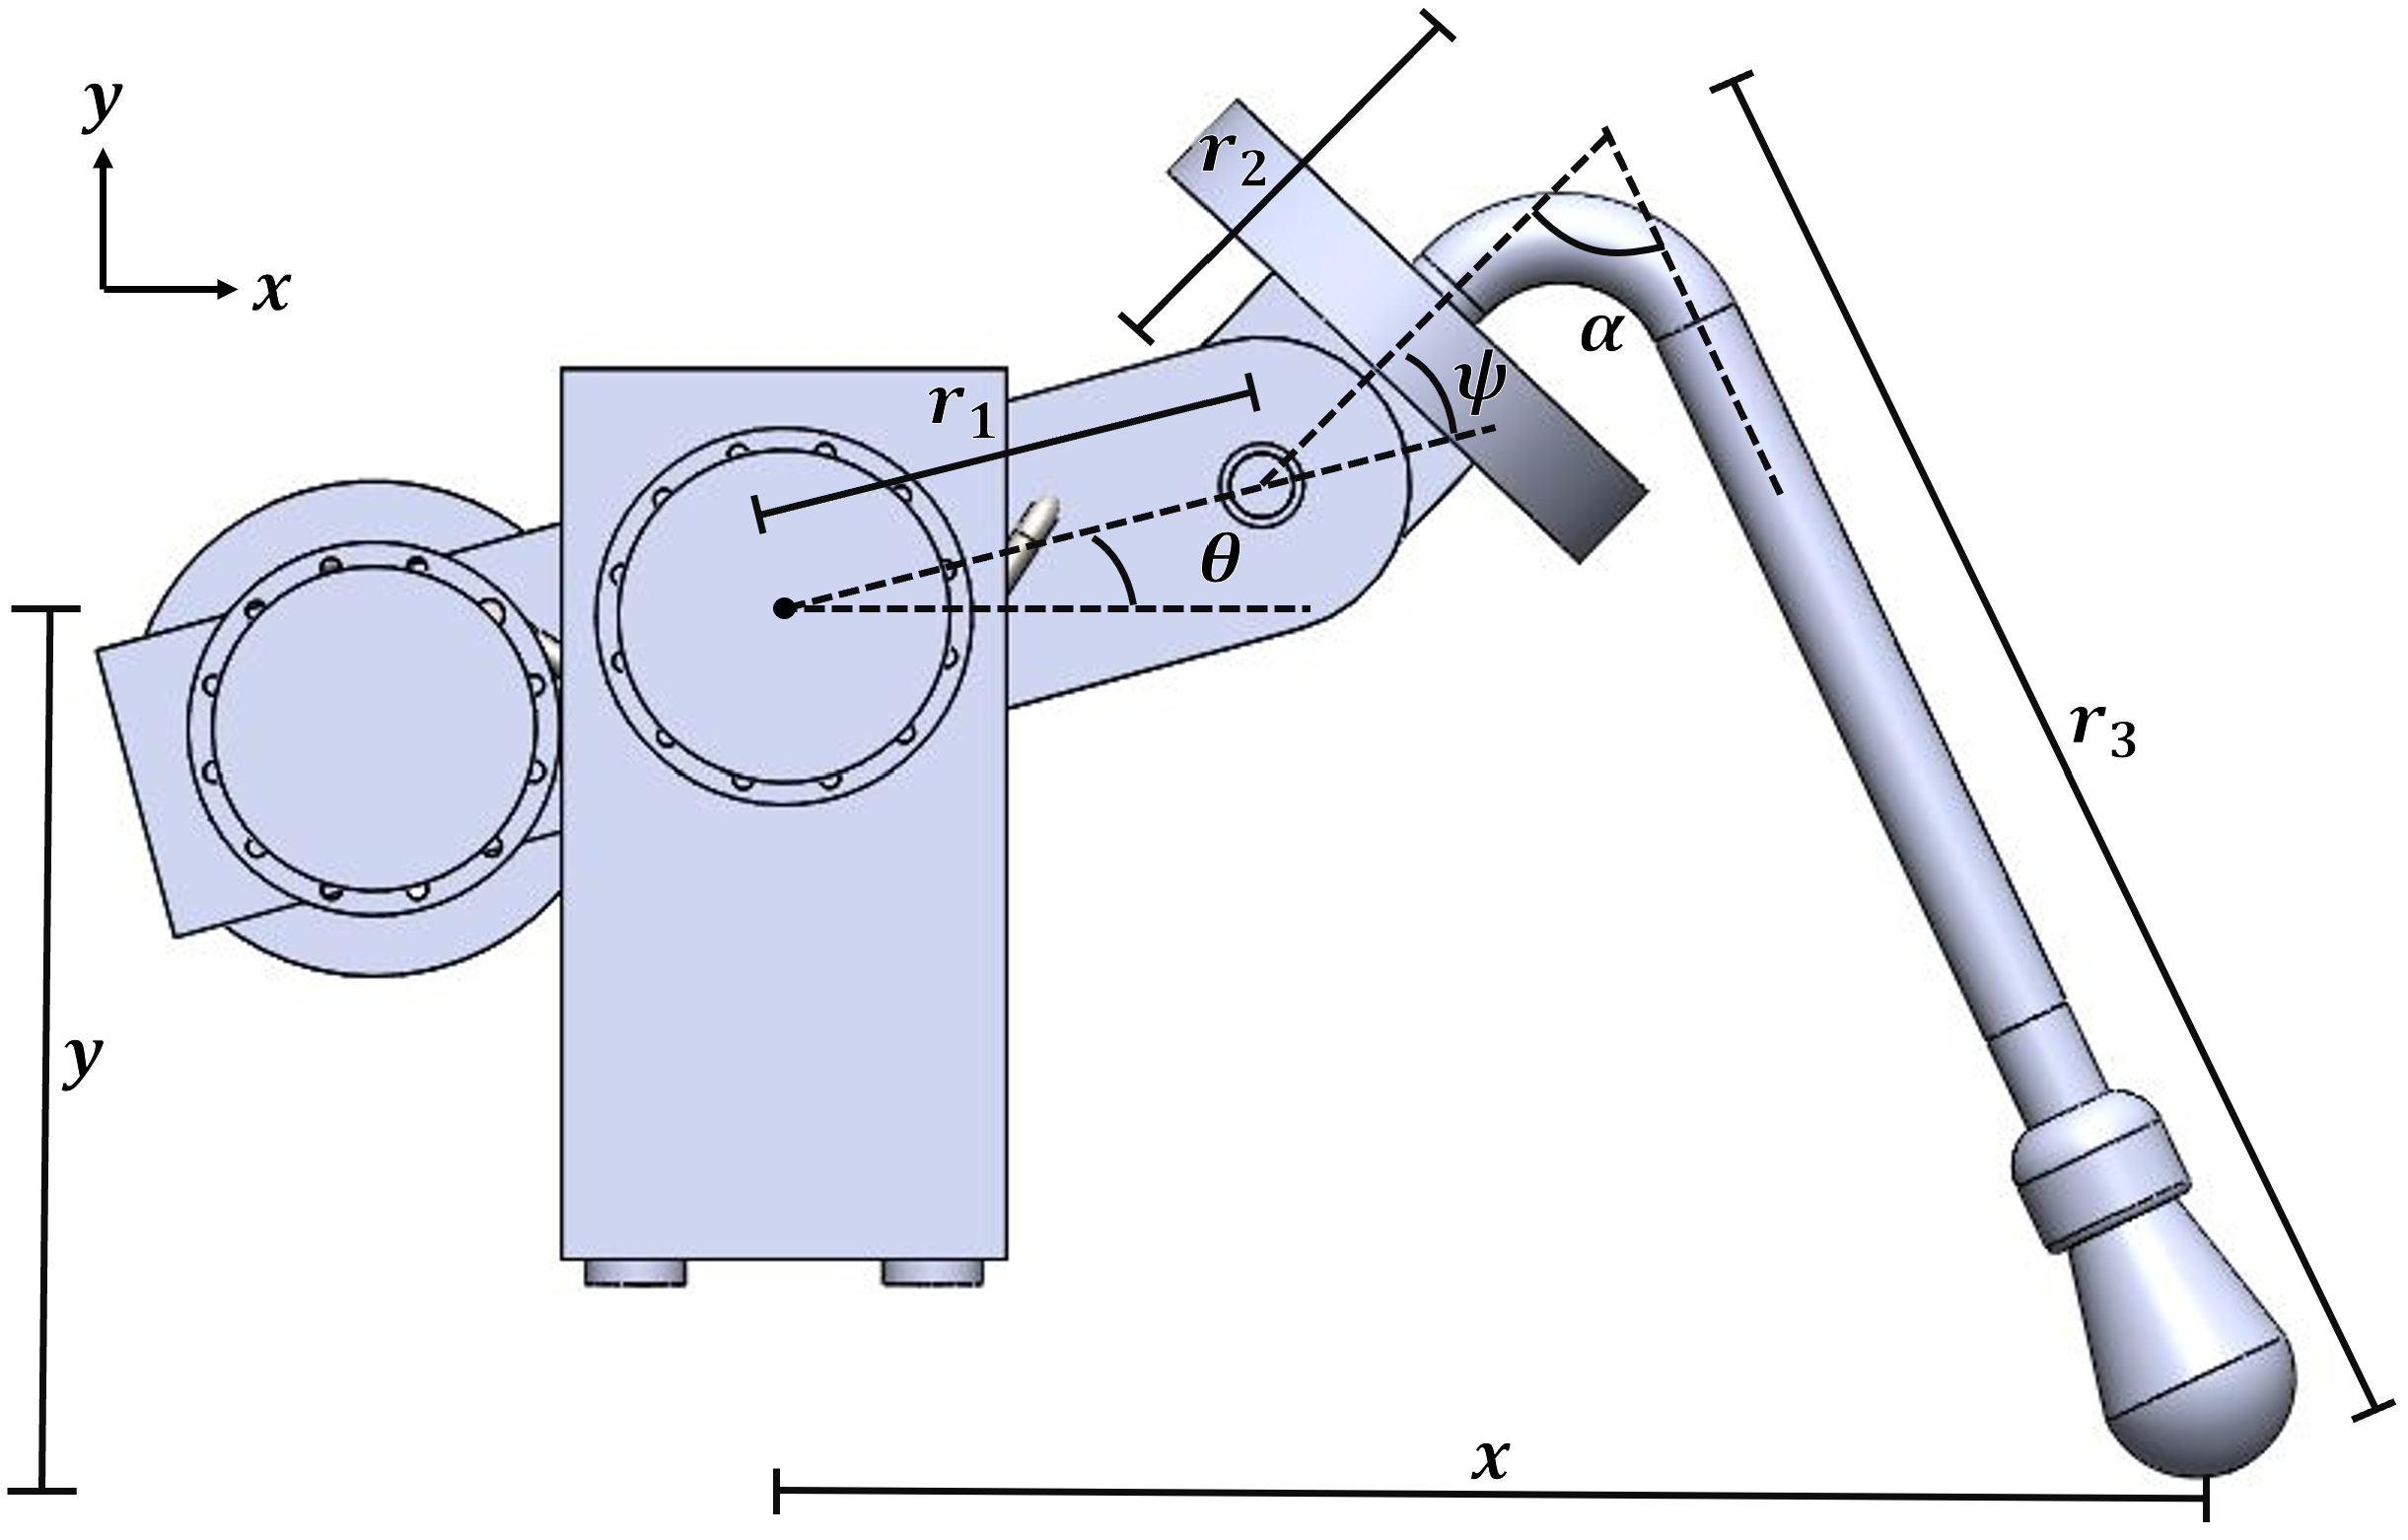
\includegraphics[width=\textwidth]{3_SystemModelling/img/LinkageOptimizationDiagram.png}
    \caption{Linkage Optimization lengths and angles}
    \label{fig:linkage_optimization_diagram}
\end{figure}{}


Ranges of $r_2$ and $\alpha$ are generated, and all permutations are run through the following steps:

\begin{enumerate}
    \item Begin with $\theta = 45^{\circ}$ and $\psi = -22.5^{\circ}$; this position gives the "ground contact height" ($d$) shown in Figure \ref{fig:linkage_optimization_steps}, as well as the closest the foot can get to the body ($x_{min}$)
    \item Increase to $\psi = 22.5^{\circ}$. This position gives the highest the leg can reach ($y_{max}$)
    \item Decrease $\theta$ until the ground is reached, giving $x_{max}$
\end{enumerate}{}

The results were then plotted in 3D, shown in Figure \ref{fig:linkage_optimization}, and a configuration that gave equal $x_{range} = x_{max} - x_{min}$ and $y_{range} = y_{max} - y_{min}$ was determined visually.
This method does not necessarily give the most optimal solution, as there is no guarantee that the furthest position the leg can reach in $x$ is with $\psi = 22.5^{\circ}$ (once $\alpha$ reaches a certain angle, $\phi$ must be lowered to touch the ground, even with $\theta = 0$).
As shown in Figure \ref{fig:linkage_optimization_steps}, the foot can technically reach further in $x$ than the found value, just at a different height $y$.
Additionally, setting different maximum and minimum angles for $\psi$ may have also provided better results.
The configuration giving a "square workspace" was $r_2=50mm$, $r_3=300mm$ and $\alpha=69^{\circ}$, giving $x_{range} = 103mm$, $y_{range} = 103mm$, and the height of the hip joint from the ground $d=190mm$.
The length $r_2$ was then found to be too small for mounting the bellow; it was doubled to 100mm, with the ranges changing to $x_{range}=97.60mm$ and $y_{range}=147.51mm$.
During parametrization, the maximum reach in $x$ and $y$ will be decided by the user; the values of $r_1$, $r_2$, $r_3$ and $\alpha$ will scale relative the the maximum desired reach.

\begin{figure}
    \centering
    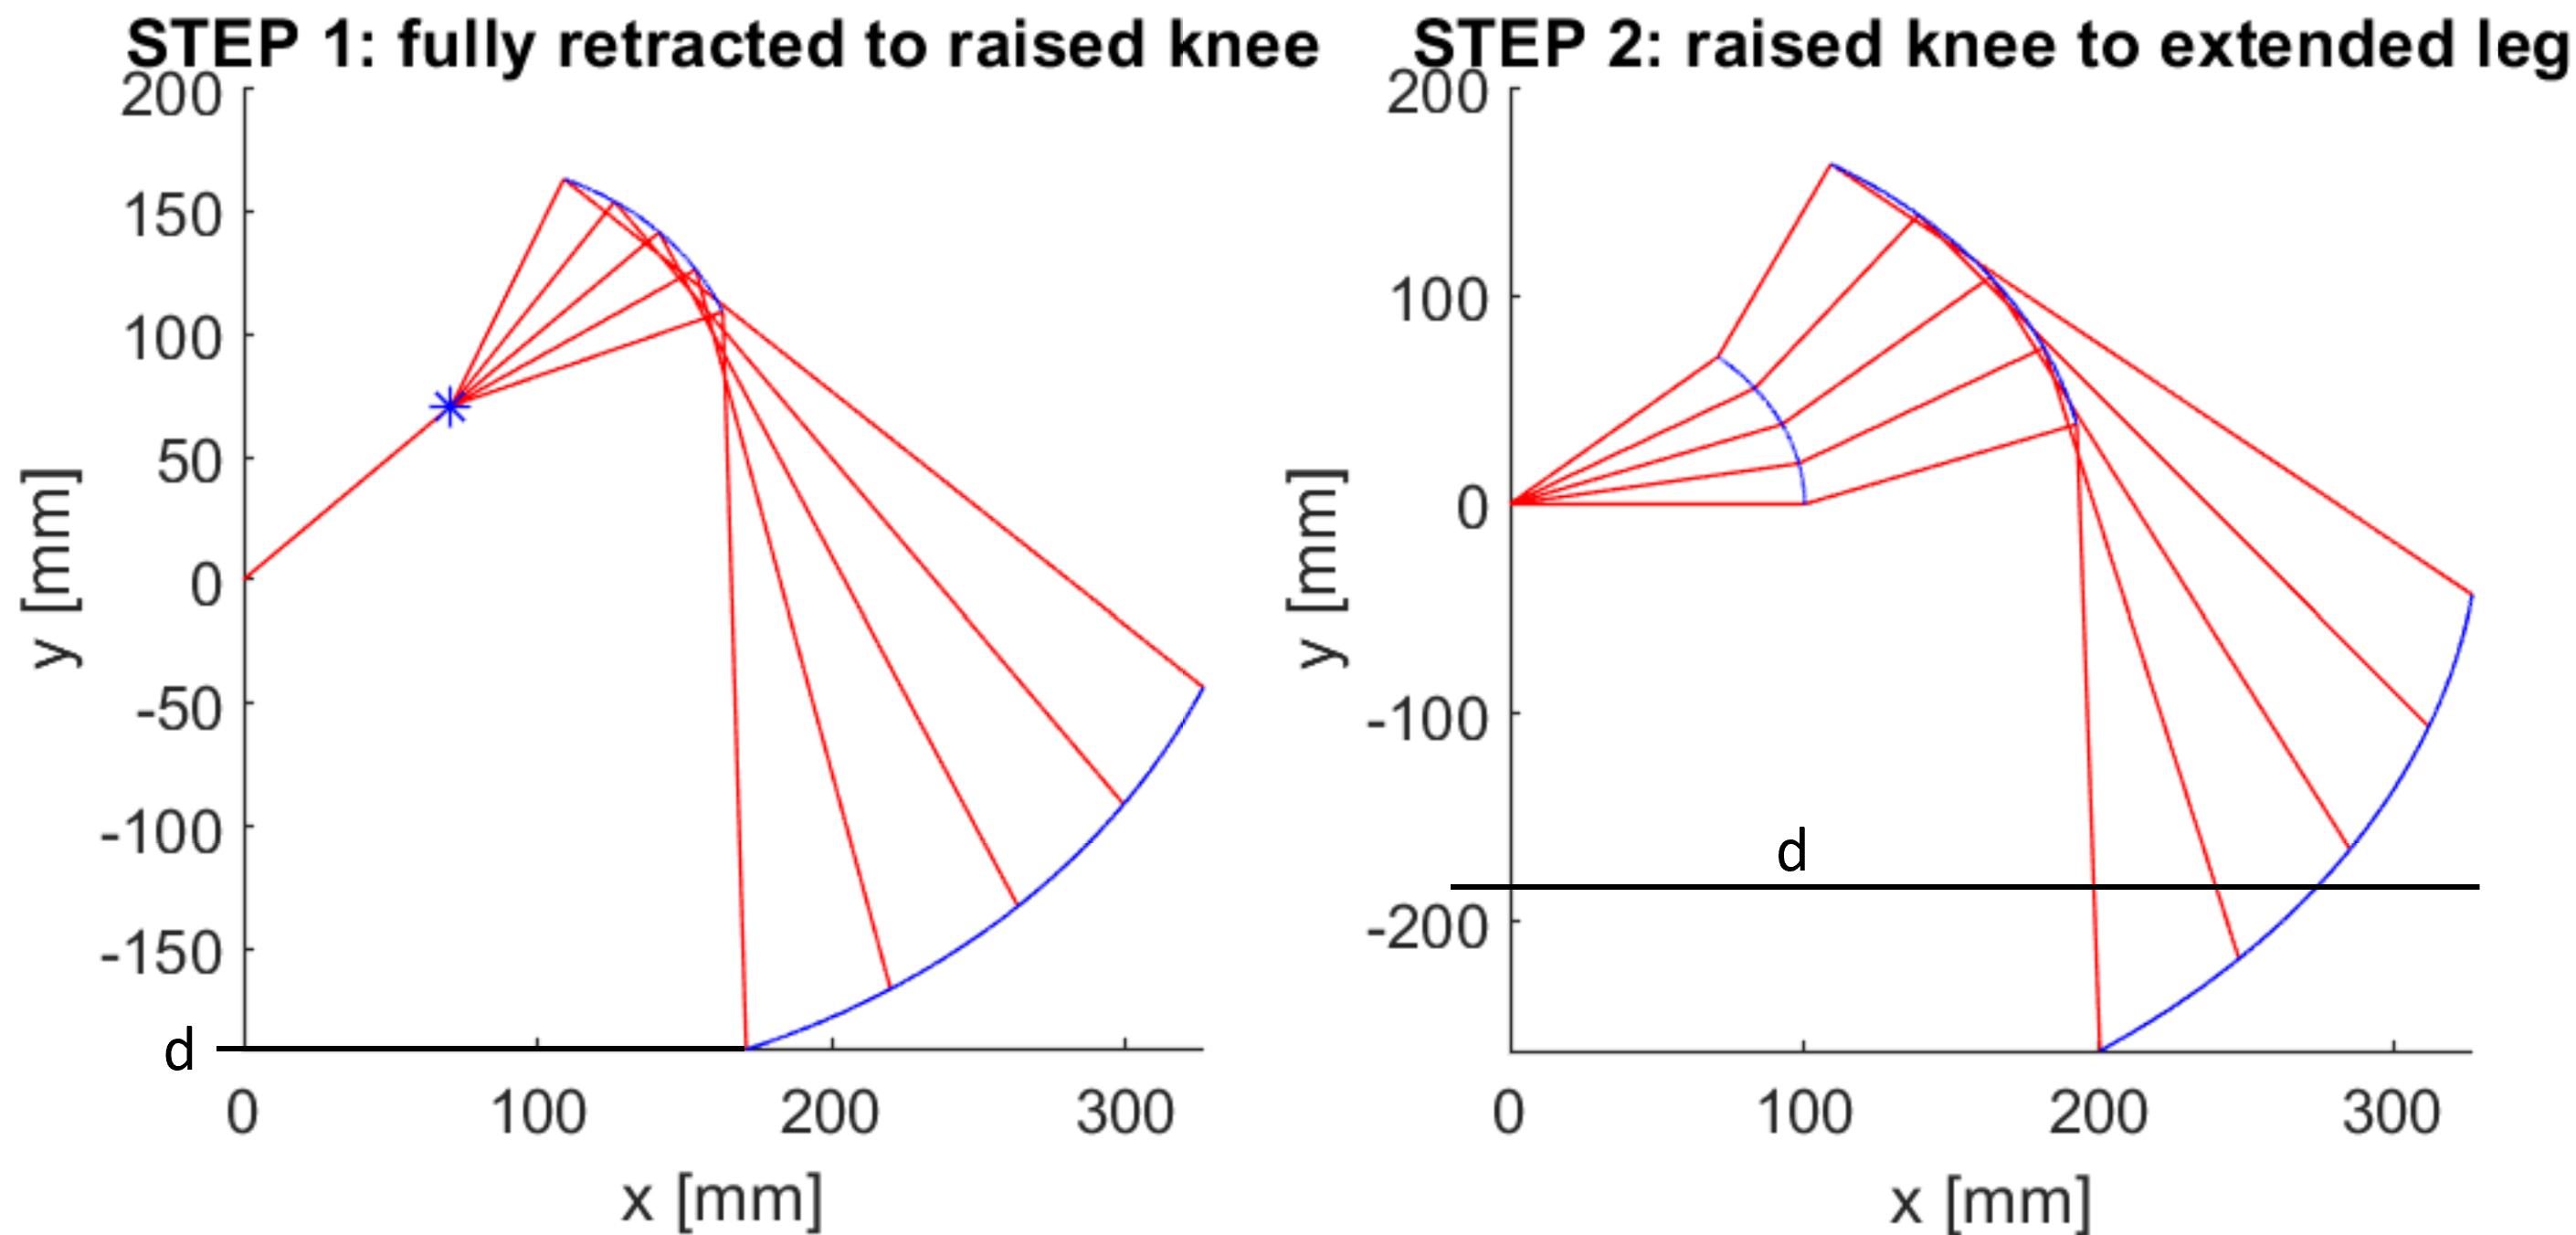
\includegraphics[width=0.7\textwidth]{3_SystemModelling/img/LinkageOptimizationSteps.png}
    \caption{Visualization of leg going through leg lifting and putting down motion, as well as ground height $d$}
    \label{fig:linkage_optimization_steps}
\end{figure}{}

\begin{figure}
    \centering
    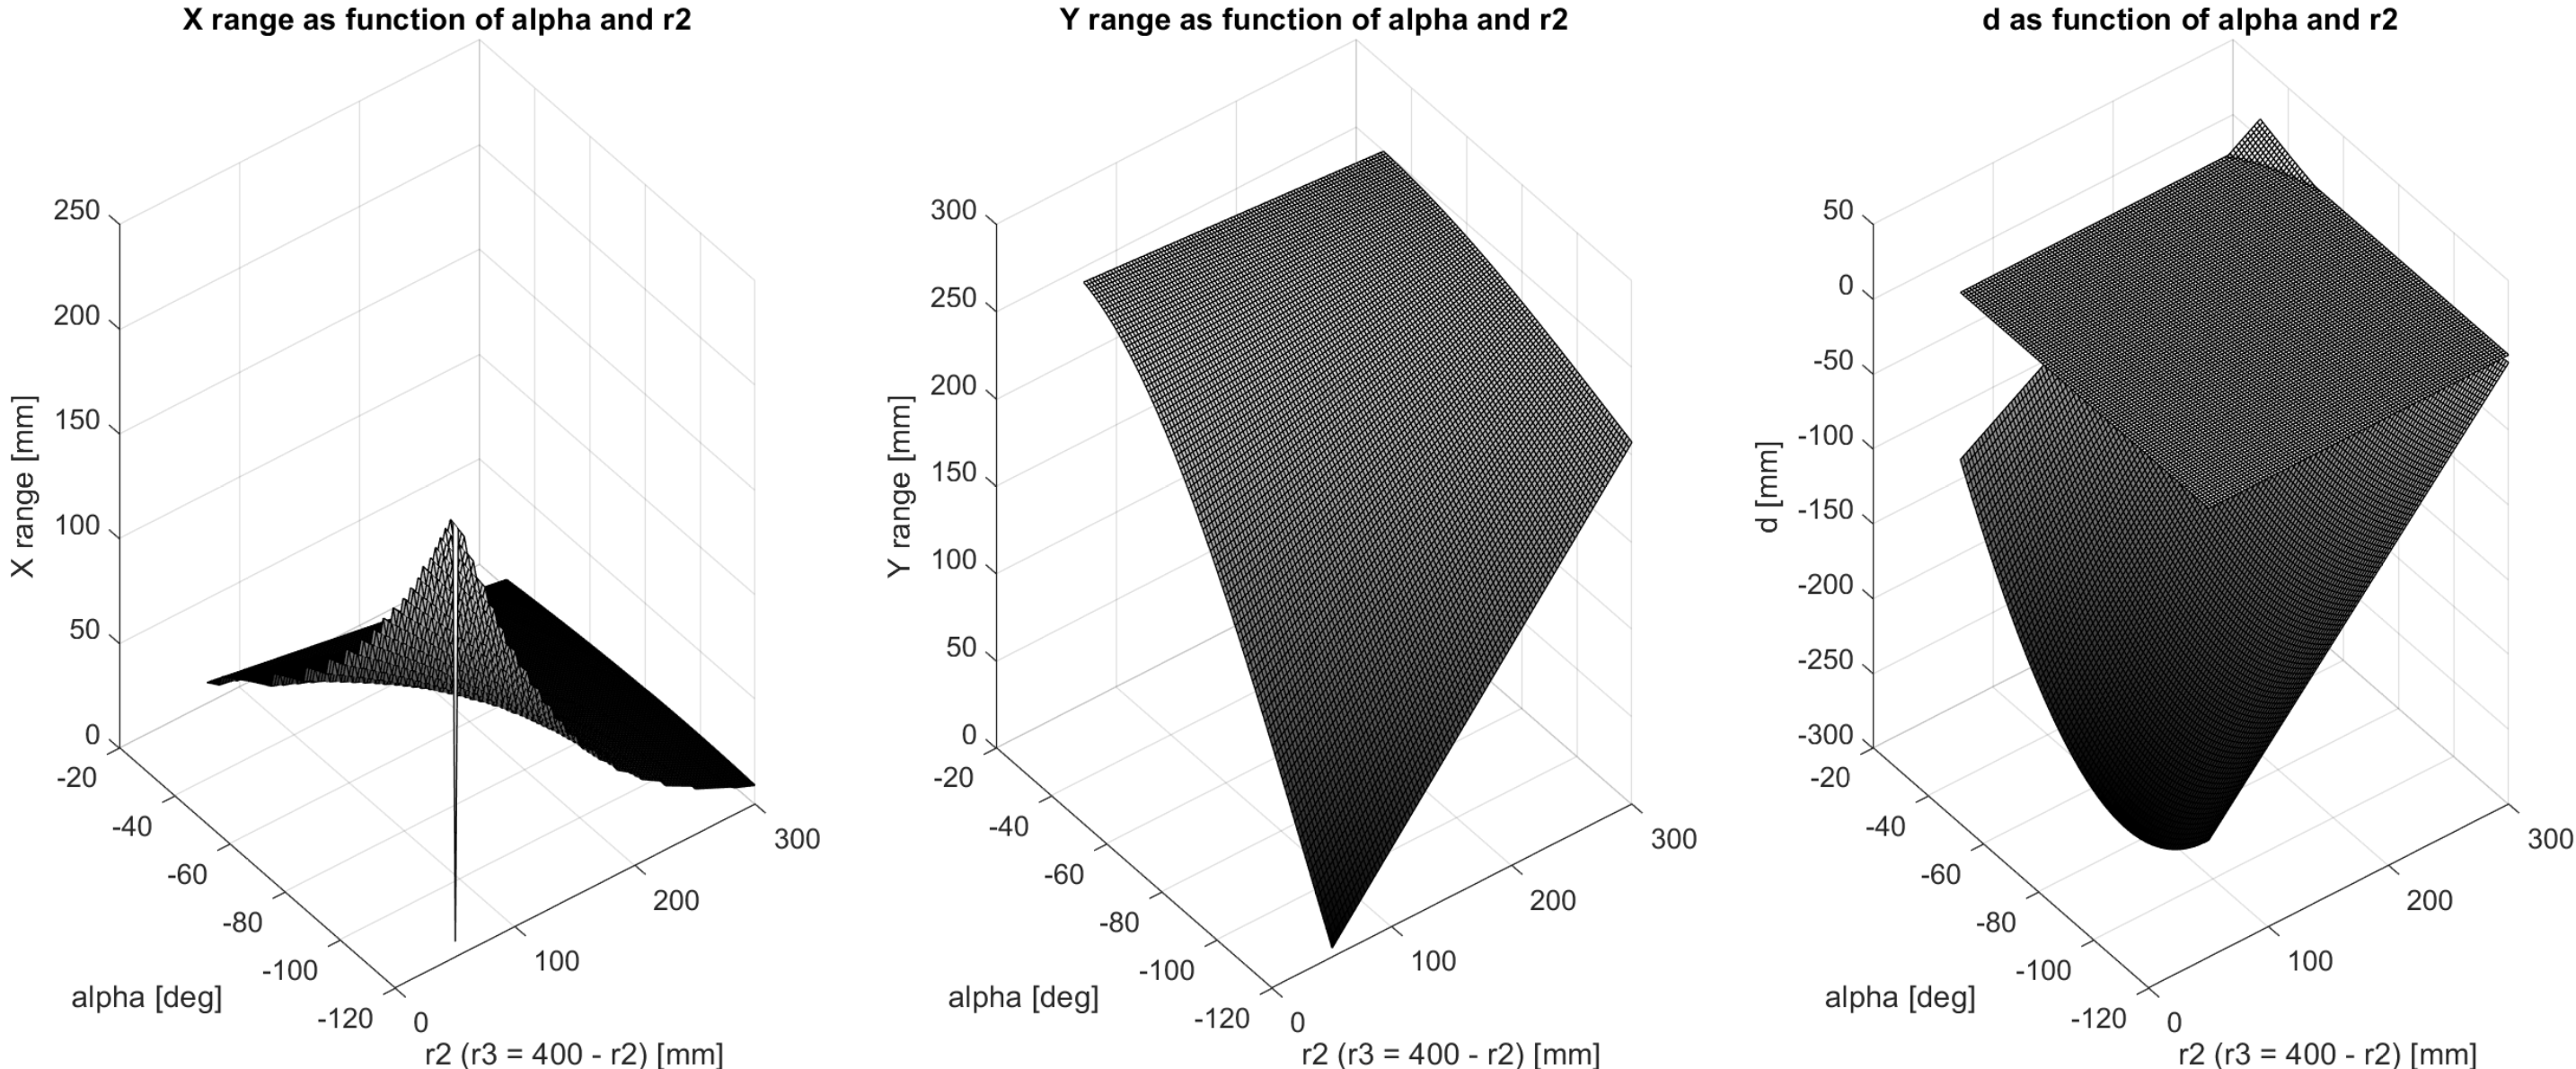
\includegraphics[width=\textwidth]{3_SystemModelling/img/LinkageOptimization3D.png}
    \caption{3D plots of range in $x$, $y$ and height from ground $d$ as functions of tibia angle $\alpha$ and linkage lengths $r_2$ and $r_3$}
    \label{fig:linkage_optimization}
\end{figure}{}


%------------------------------ POWER CONSUMPTION ------------------------------%
\subsection{Power Consumption} \label{subsec:power_consumption}

\subsubsection{Harmonic Drives Efficiency} \label{subsubsec:HD_efficiency}

The Harmonic Drive and motor at the hip for the heaviest and largest robot were selected to demonstrate the following equations.
The example uses the average output speed and half of peak torque seen by the drive.
Specifications will appear as used.
Harmonic Drive efficiency depends on the input rotation speed and ratio of output torque to rated torque \cite{harmonic_drive_csd-2a_2019}.
The speed efficiency $\eta_r$ was extracted from Harmonic Drive's website using Engauge Digitizer and is approximated using MATLAB's curve fit tool.

\begin{equation}
    \begin{split}
        \eta_r = 4.848\times10^{-9} (rpm_{motor})^2 -5.879\times10^{-5} (rpm_{motor}) + 0.8367
        \\
        = 4.848\times10^{-9} (237.77\text{rpm})^2 -5.879\times10^{-5} (237.77\text{rpm}) + 0.8367 = 0.823
    \end{split}{}
\end{equation}

where $rpm_{motor}$ is the output speed of the motor in rotations per minute (RPM).
Harmonic Drive only gives values of $0.69 < eta_r < 0.81$, so the result will be limited to this range ($\eta_r=0.81$).
The torque efficiency depends on

\begin{equation}
    \alpha = \frac{\text{load torque}}{\text{rated torque}} = \frac{18.61\text{Nm}}{37.23\text{Nm}} = 0.5
\end{equation}{}

where the rated torque is the L10 rated torque provided by Harmonic Drive.
The torque efficiency is found in the same was as the speed efficiency and approximated as

\begin{equation}
    \begin{split}
        k_e = -1.481\alpha^4 + 4.312\alpha^3 - 5.013\alpha^2 + 3.159\alpha - 0.02076
        \\
        = -1.481(0.5)^4 + 4.312(0.5)^3 - 5.013(0.5)^2 + 3.159(0.5) - 0.02076 = 0.75
    \end{split}
\end{equation}{}

Finally, the overall efficiency of the Harmonic Drive is given by

\begin{equation}
    \eta_{HD} = \eta_r k_e = (0.823)(0.75) = 0.61
\end{equation}{}

The input torque to the Harmonic Drive (and thus output by the motor) is given by

\begin{equation}
    T_{m} = \frac{T_{HD}}{\eta_{HD} e} = \frac{18.61\text{Nm}}{(0.61)(100)} = 305.63\text{mNm} = 305.63\text{Nmm}
\end{equation}{}

where $e$ is the gear ratio of the Harmonic Drive (chosen for our project to be 100).


\subsubsection{Motor Power Consumption} \label{subsubsec:power_motor}

Maxon Motor provides equations relating the power in and out of the motor, and power losses \cite{maxon_motor_maxon_2014}.
Rearranging these equations provides us with the voltage of the motor

\begin{equation}
    \begin{split}
        U = \frac{1}{k_s} \left(\frac{30000R_m T_m}{\pi k_T^2} + \omega_m\right) = \frac{1}{81.31\frac{\text{rpm}}{V}} \left(\frac{30000(2.96\Omega) (305.63\text{Nmm})}{\pi (117.43\frac{\text{Nmm}}{A})^2} + (237.77\text{rpm})\right) 
        \\
        = 10.62\text{10.62V}
    \end{split}
\end{equation}{}

where $k_s \left[\frac{RPM}{V}\right]$ is the speed constant, $k_T \left[\frac{mNm}{A}\right]$ is the torque constant, $R_m [\Omega]$ is the motor resistance and $\omega_m = \omega_{HD} e [RPM]$ is the output speed of the motor.
The motor current can be solved for using the quadratic equation with $a=R_m =2.91\Omega$, $b=-U =-10.62\text{V}$ and $c=\frac{\pi \omega_m T_m}{30000}=\frac{\pi (237.77\text{rpm})(305.63\text{Nmm})}{30000}=7.61$.
If the motor speed is 0, then the lower result gives 0 and the larger result should be taken.
Otherwise, the smaller result should be taken (for a motor running near nominal conditions, the lower result of the quadratic equation will give very close to the nominal current whereas the upper value will give an answer an order of magnitude higher).
For the given instance, $I = 0.9876\text{A}$.


\subsubsection{Robot Power Consumption} \label{subsubsec:power_simulation}

An inaccurate method of calculating robot power consumption is to sum the nominal current of all motors (and electronics), and treat the total current as being continuously drawn.
As our design allows for springs and Harmonic Drives to take the robot's weight during rest, as well as the robot gait only moving one leg forward at a time, a more accurate method is required to allow significant battery size and robot weight reductions.
A simulation was written that splits the gait into 3 phases.
The steps for a front leg are:

\begin{enumerate}
    \item The leg starts fully retracted ($\theta=45^{\circ}$ and $\phi=-22.5^{\circ}$). Phi moves from its bottom position to its top position ($\phi=22.5^{\circ}$).
    \item The leg lowers by reducing $\theta$ until the foot makes contact with the ground (a position determined in \ref{subsec:linkage_optimization})
    \item The leg pulls the body forward until reaching the position from the beginning of phase 1
\end{enumerate}{}

The steps for a rear leg are the opposite.
While one leg is performing steps 1 and 2, the other 4 legs remain stationary, and while close to the body the legs consume no power.
The simulation ran over each phase for each leg and summed the coulombs expended at each step based on the output speed and torque, joint angles, and Harmonic Drive and motor calculations presented in Subsections \ref{subsubsec:HD_efficiency} and \ref{subsubsec:power_motor}.
The total number of coulombs was summed and divided by the simulation time to give the average amperage during walking.
The code can be found in Appendix \ref{app:code_power_consumption}.
For the heaviest and largest predicted robot, with a body mass of 30kg and leg geometry taken from \ref{fig:linkage_optimization}, consumes on average 5.4A.
The other electronics (Raspberry Pi, NVIDIA Jetson, drivers, sensors, etc.) collectively consume 2.13A, giving a total system power draw of 7.55A.
Since the batteries output at 48V for the motors, the total power consumption is

\begin{equation}
    P = (7.55A)(48V) = 362.4W
\end{equation}{}

\subsubsection{Solar Power} \label{subsub:solar_power}

A typical day in Ottawa during the summer will emit solar radiation similar to Figure \ref{fig:solar_radiation}. As solar radiation emission will vary greatly with weather, two days were taken into account, July 1st 2019 as shown in Figure \ref{fig:solar_radiation} and July 17th 2019. The mean $KJ/m^2$ for both days was taken to calculate a more realistic solar radiation average. The average was calculated as $2111.273 KJ/hm^2$.

\begin{figure}
    \centering
    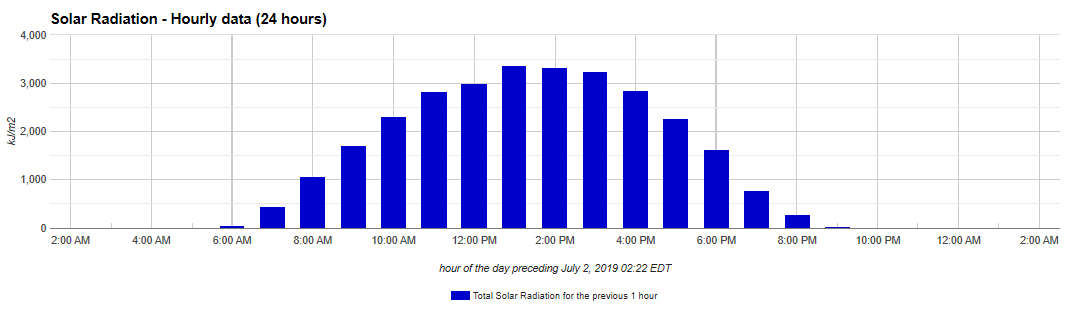
\includegraphics[width=\textwidth]{3_SystemModelling/img/SunCalculation.PNG}
    \caption{Hourly Solar Radiation Emission - Ottawa July 1st 2019 \cite{environment_and_climate_change_canada_solar_nodate}}
    \label{fig:solar_radiation}
\end{figure}{}


The total watts produced is calculated using the equation below and where $S$ is the radiation emission in $KJ/hm^2$, $\mu$ is the solar panels efficiency \cite{sunpower_solar_2018} and $A$ the area of solar panels on the robot. 

\begin{equation}
    W_{absorbed} = \frac{S \mu A }{(3600 s/h)} = \frac{(2111.273 \frac{KJ}{h m^2})(0.223)(0.5 m^2)}{(3600 s/h)} = 65.39 W
\end{equation}

As a constraint, the robot's batteries must be completely recharged by the end of the day. Thus, the total amount of energy consumed by the robot during the day must be compensated by the solar energy absorbed. The robot requires 355 Watts of power, and according to the calculations above will absorb 65 Watts. Using the equation below, the total run time capability of the robot is calculated by:

\begin{equation}
    R = \frac{W_{absorbed} H}{W_{consumed}} = \frac{(65.39W)(10h)}{(362.4W)} = 1.80 h
\end{equation}

where R is the total runtime in hours, H the number of hours of sun during the day. The robot can only accomplish throughout the day 1.8 hours of work time if it is to only use the energy it can absorb.

\subsubsection{Battery} \label{subsub:battery}

Cells are arranged into a battery and managed by a Battery Management System \cite{voltaplex_6s16s_nodate}. All electronics are powered from this with the necessary voltage regulators.
The battery voltage is defined as the highest voltage of any component, $V_{max}$, which is the motors running at 48 V.
The number of battery cells running in series, $N_{series}$, is defined as

\begin{equation}
    N_{series} = \frac{V_{max}}{V_{cell}} = \frac{V_{max}}{3.6 V} = \frac{48V}{3.6V} = 14 \text{ cells}
\end{equation}

The number of cells in parallel, $N_{parallel}$, to achieve the desired run time is defined as

\begin{equation}
    N_{parallel} = \frac{T \cdot I}{Q} = \frac{(1.8h)(7.55A)}{3.4Ah} = 4 \text{ cells}
\end{equation}

where $T$ is the runtime in hours, $I$ is the total current draw of the robot and $Q$ is the Amp-hour rating of an individual battery cell \cite{digikey_electronics_battery_nodate}.
The total number of required cells is the number of series cells multiplied by the number of parallel cells.

\begin{equation}
    N = N_{parallel} \cdot N_{series} = 4\times 14 = 56
\end{equation}

\subsubsection{Results of Power Consumption Simulation}

Using the code given in Appendix \ref{app:code_power_consumption}, the average current draw is found to be 7.53A.
This results in four cells in parallel for 1.8 hours of battery life and 14 cells in series to match the 48V of the motor, giving a total of 56 cells.
At 50g each, the combined weight of the cells is 2.8kg, far down from the approximately 238 cells needed when constantly running at nominal current (or 11.9kg) \cite{18650batterystore_18650_nodate}.
The more accurate method of calculating power consumption in Section \ref{subsubsec:power_simulation} reduces the battery mass by two thirds over the naive approach.